\documentclass[11pt]{amsart}

% Standard letter size paper with 1inch margins
\usepackage[letterpaper, margin=1in]{geometry}

% Useful packages 
\usepackage{amsmath, amssymb, amsthm, amsaddr}
\usepackage{enumerate, subcaption, graphicx, hyperref}
\usepackage{algorithm}
\usepackage{algpseudocode}
\usepackage{cite}

\newcommand{\I}{\mathrm{i}}
\DeclareMathOperator{\E}{e}

\title{AMATH 582: Homework 2}
\author{Hunter Lybbert} % first and last name

\address{Applied Mathematics Department, University of Washington, Seattle, WA 
\\ \texttt{hlybbert@uw.edu}}

\date{\today} % you can also just type the date instead of "\today"

\begin{document}

\maketitle

\begin{abstract}
    This is my Abstract \textbf{TODO}
\end{abstract}

\section{Introduction and Overview}\label{sec:Introduction}
This is my Introduction \textbf{TODO}
In order to understand the data and attempt to classify the movements of the robot we aimed to complete the following 5 tasks: \\
\begin{enumerate}
\item Through \textbf{averaging of the Fourier transform} determine the dominant frequency (center frequency)
generated by the submarine. Verify your results through visualization. \\

\item Design and implement a \textbf{Filter} to extract this center frequency in order to denoise the data and
determine a more robust path of the submarine. Visualize the denoised measurement the 3D path of
the submarine and inspect the validity and effectiveness of the denoising. \\

\item Determine and \textbf{plot the} $x$-$y$ coordinates of the submarine path during the 24 hour period. This
information can be used to deploy a sub-tracking aircraft to keep an eye on your submarine in the future.

\end{enumerate}

In the endeavor to reduce the dimensionality of the robot movement data, classify the movements, and complete the requisite tasks, we made extensive use of several important Python packages.
Namely, Matplotlib was used to create all plots and animations \cite{Hunter:2007}.
Additionally, Scikit-learn was the primary source of using the PCA algorithm and other classification methods \cite{scikit-learn}. 
Finally, NumPy was once again a crucial tool \cite{harris2020array}.
Moreover there are important theoretical underpinnings behind the algorithm we implemented which will be cited and expounded upon in the following section.

\section{Theoretical Background}\label{sec:theory}
Technical background duh duh duh ... \textbf{TODO}

\begin{equation}
X = U\Sigma V^T
\label{eq:svd}
\end{equation}

Let's get into the actual implementation now.

\section{Algorithm Implementation and Development}\label{sec:algorithms}
We will now describe in words and pseudocode the implementation of these methods as we used them in this application to reduce the dimensions of our data and try to preserve as much information as possible.
First, we discuss the PCA algorithm in \ref{alg:pca_alg}.

\begin{algorithm}
\caption{Determine the Dominant Frequency}\label{alg:pca_alg}
\begin{algorithmic}
\State $ S = {\rm np.load(data)}$ \Comment{Input subdata, after reshaping to (64, 64, 64, 49)}
\State $\hat S$ = fftn(S)
\State $\hat S^\dag$ = fftshift($\hat S$) \Comment{Transformed and shifted subdata (64,64,64,49)}

\State $\hat S^\dag_{\rm avg} = {\rm avg}(\hat S^\dag)$ \Comment{Average computed across time at each point (64,64,64)}
\State $x, y, z = {\rm argmax} \left( {\rm abs} \big( \hat S^\dag_{\rm avg} \big) \right) $ 
\end{algorithmic}
\end{algorithm}

The result of the final step of Algorithm \ref{alg:pca_alg} are \textbf{TODO: fill in deets}.
What we really want is to know what the frequency value should be to center our gaussian filter from equation \eqref{eq:svd} to use in Algorithm \ref{alg:classification}

\begin{algorithm}
\caption{Apply Gaussian Filter in Frequency Space}\label{alg:classification}
\begin{algorithmic}
\State $ G = \frac {1}{\sqrt{2 \pi \sigma^2}}\exp \Big( - \frac{1}{2 \sigma^2 }\big(k_x - k_{x_0}\big) + \big(k_y - k_{y_0}\big) + \big(k_z - k_{z_0}\big) \Big)$ \Comment{Gaussian Filter using \eqref{eq:svd}}
\State $\hat S$ = fftn(S)
\State $\hat S^\dag$ = fftshift($\hat S$)
\State $\hat F^\dag = \hat S^\dag G$ \Comment{Filtered subdata in frequency space still}
\State $\hat F = {\rm ifftshift}(\hat F^\dag)$
\State $F = {\rm ifftn}(\hat F)$ \Comment{Filtered subdata in signal space now}
\end{algorithmic}
\end{algorithm}

\textbf{TODO:}. These results will be described further in following section.

\section{Computational Results}\label{sec:results}
We have the following to talk about:
\begin{itemize}
\item Talk about getting the right shape for training
\item That means we had to treat each frame of the robot movements as a single sample
\item Talk about the classification issues
\item why we used the Support vector machine to try and classify more accurately
\end{itemize}

\begin{figure}[h]
	\centering
	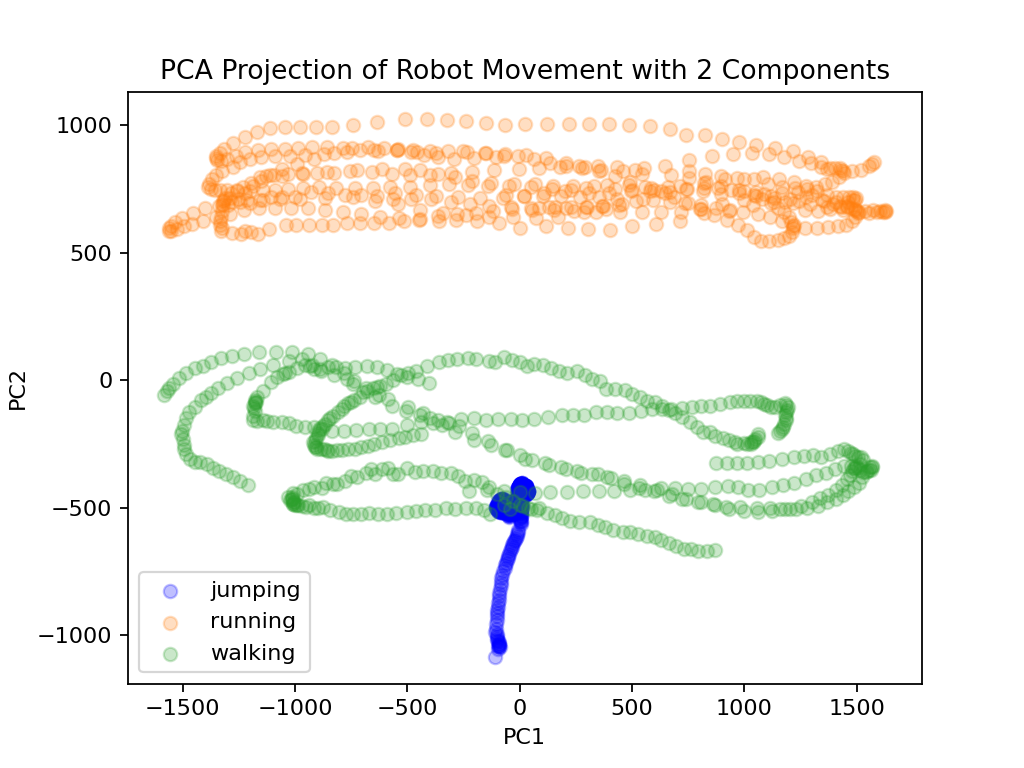
\includegraphics[width=.5\textwidth]{../visualizations/pca_2_components_plot.png}
 	\caption{Visualizing each of the 3 slices including the location in our 3 dimensional average frequency object.}\label{fig:f1_0}
\end{figure}

\begin{figure}[h]
	\centering
	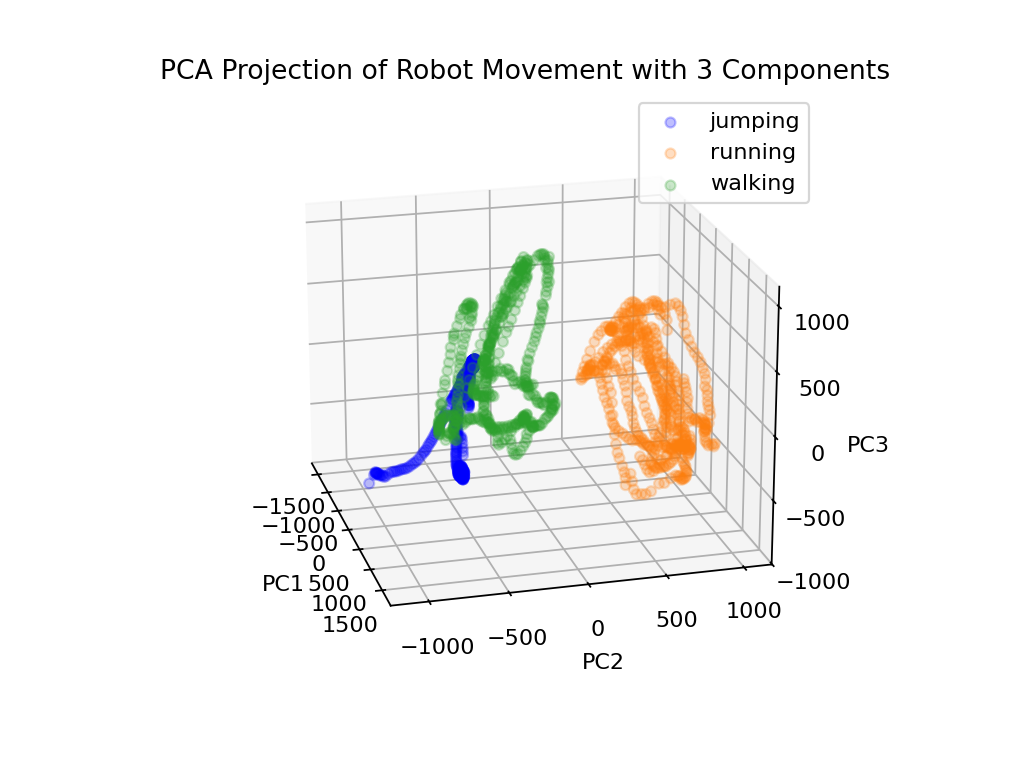
\includegraphics[width=.5\textwidth]{../visualizations/pca_3_components_plot.png}
 	\caption{Visualizing each of the 3 slices including the location in our 3 dimensional average frequency object. We also visualize a slice which does not intersect the max frequency in order to convey how drastic the location of the max frequency is. In order to show this comparison things have been rescaled here.}\label{fig:f1}
\end{figure}


As seen in Figures \ref{fig:f1_0} and \ref{fig:f1}, then Figure \ref{fig:f2}.

\begin{figure}[h]
	\centering
	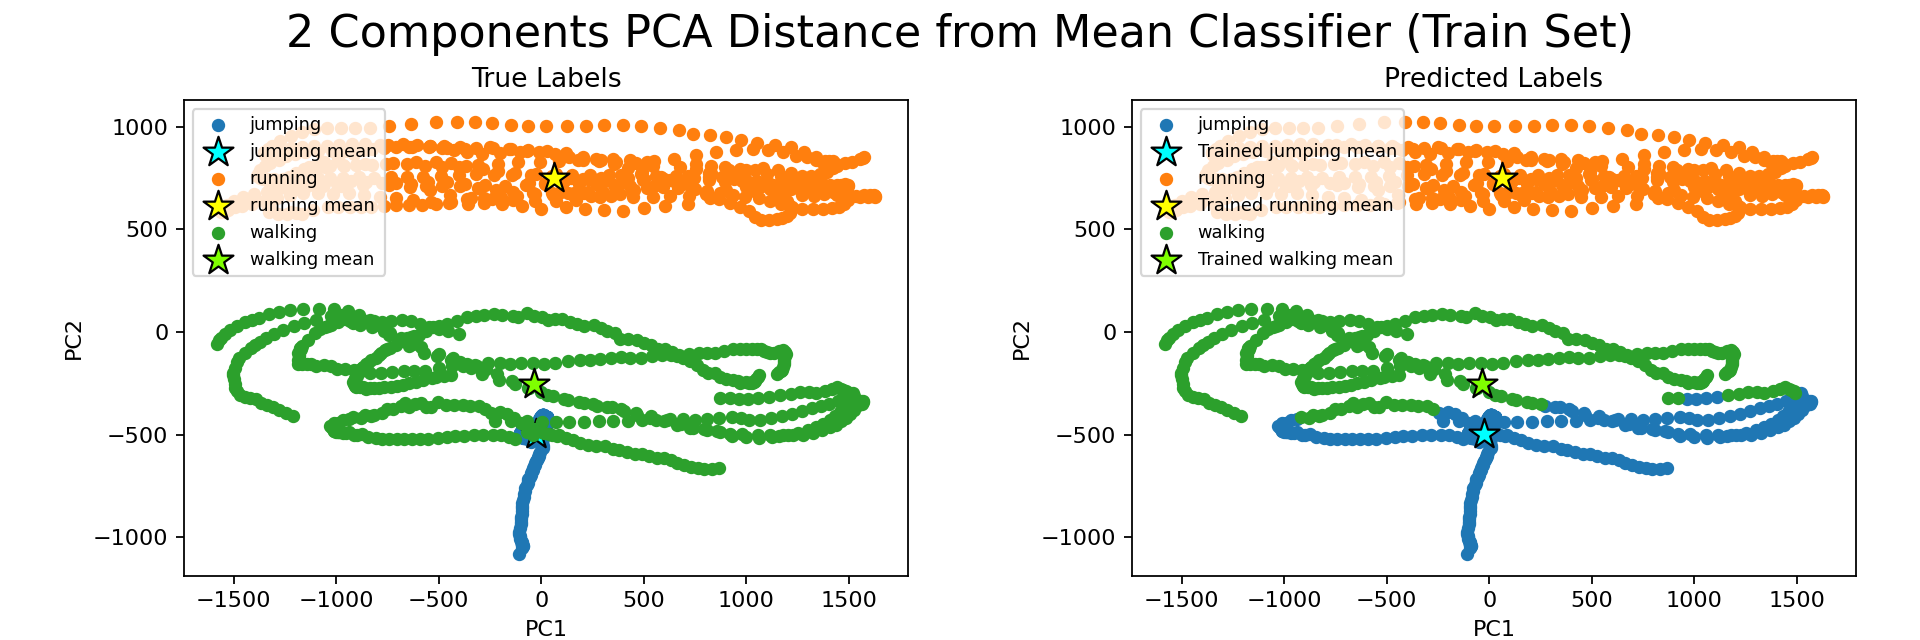
\includegraphics[height=2in]{../visualizations/pca_distance_from_mean_classifier_2d.png}
 	\caption{The resulting path in 3 dimensions that we determined after applying Algorithms \ref{alg:dom_freq} and \ref{alg:filter}. In this iteration of the filter we used $\sigma=1.3$.}\label{fig:f2}
\end{figure}

\begin{figure}[h]
	\centering
	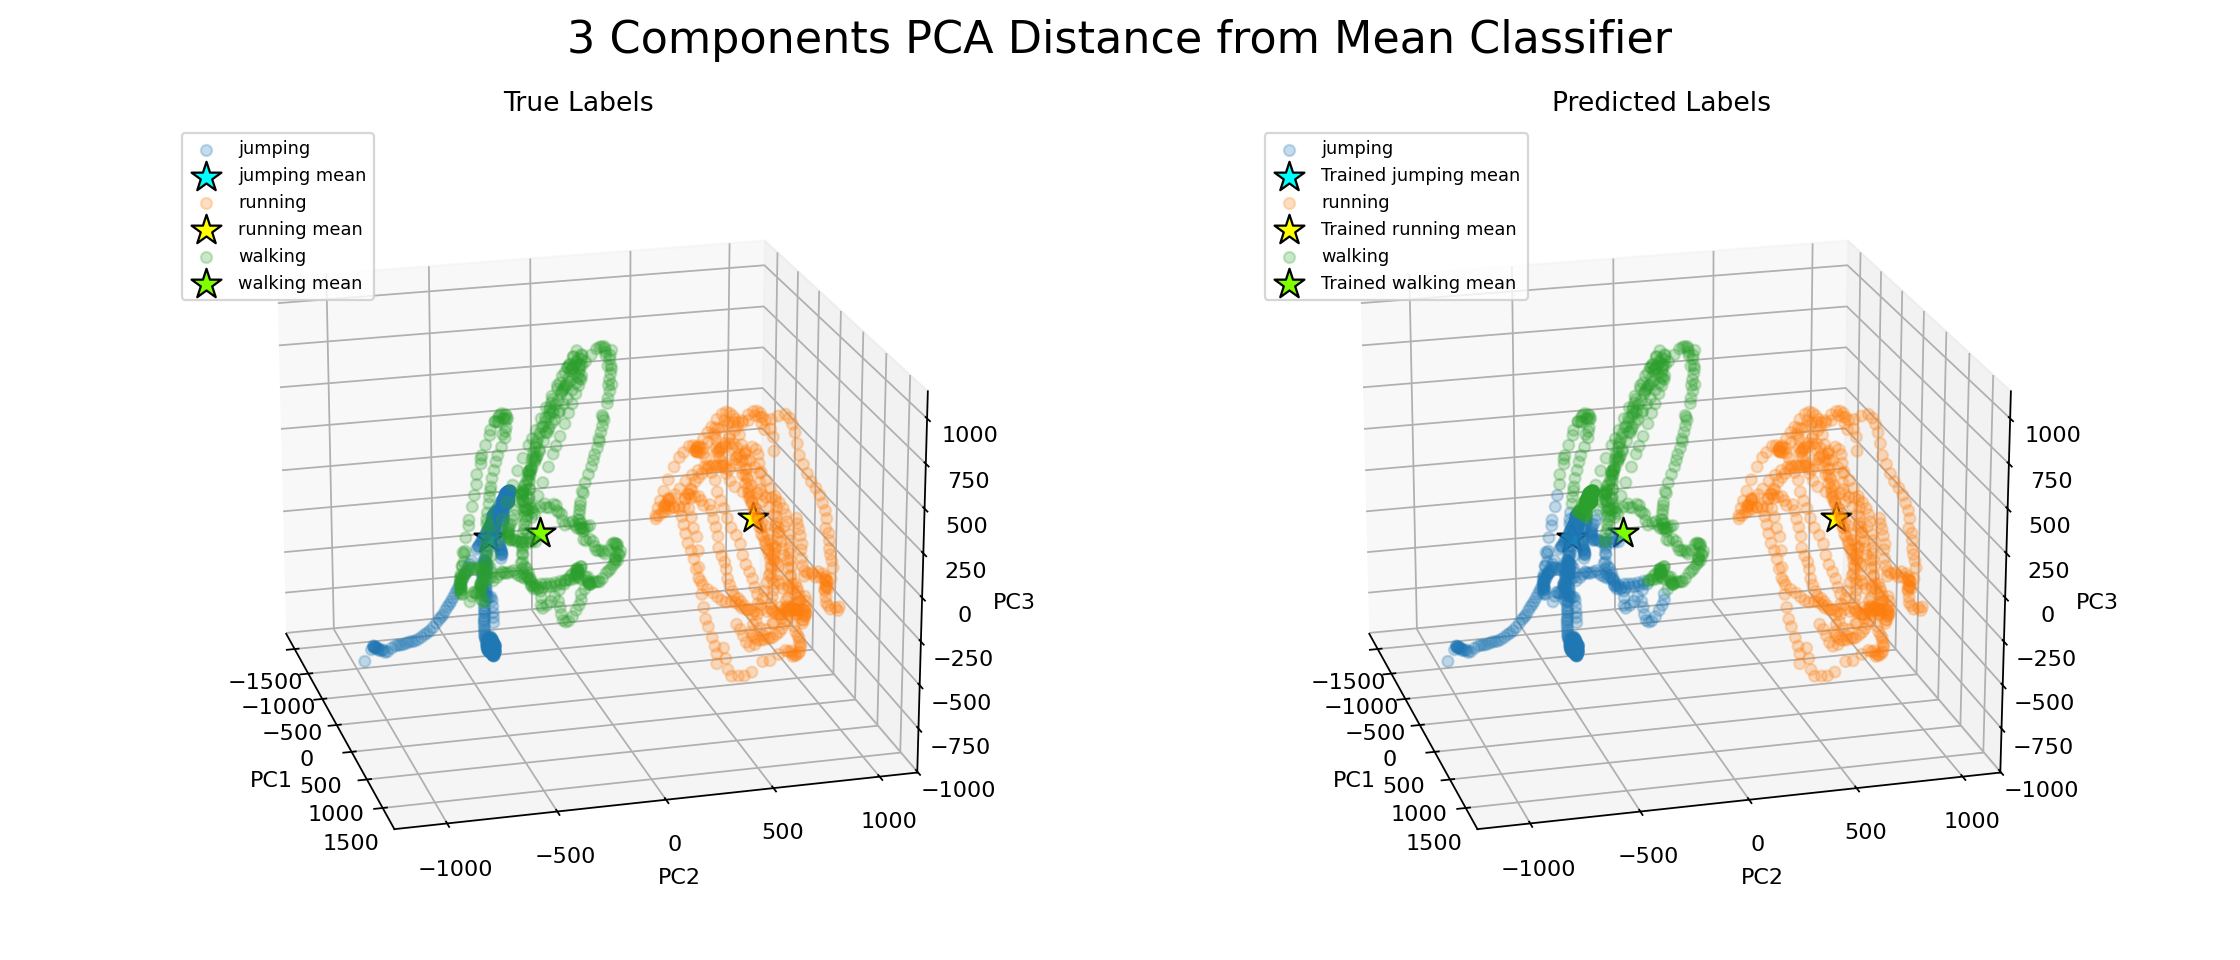
\includegraphics[height=2in]{../visualizations/pca_distance_from_mean_classifier_3d.png}
 	\caption{This is just the 2 dimensional projection of the path given in the above 3d plot. The same value of $\sigma$ was used in the filter.}\label{fig:f3}
\end{figure}

\section{Summary and Conclusions}\label{sec:conclusions}
This is my summary and conc.

\section*{Acknowledgements} 

The author is thankful to Jaxon Tuggle for useful discussions about the process to find the correct dimensions to use when interpreting the training data samples we were given.
We would also like to thank Professor Eli Shlizerman for carefully instructing us in class.
Finally, it is necessary to thank the following students Nate Ward, Sophie Kamien, whose questions helped clarify understanding of the algorithm we implemented by giving chances to explain ideas and debug code together.

\bibliographystyle{abbrv}
\bibliography{references_hw2} % make sure this matches the .bib file for your corresponding document. You also have to maintain your references in the .bib file 

\end{document}
